\documentclass[8pt, compress]{beamer}

%%% default
%\geometry{paperwidth=128mm,paperheight=96mm}

%\geometry{paperwidth=145mm,paperheight=108.75mm}
\geometry{paperwidth=175mm,paperheight=108.75mm}

%\geometry{paperwidth=150mm,paperheight=112.5mm}
%\geometry{paperwidth=160mm,paperheight=120mm}

\mode<presentation> {
  \usetheme{Warsaw}
 % \usetheme{Boadilla}  
  \setbeamercovered{transparent}
}

% make the navigation bar to disappear
\setbeamertemplate{headline}{}

%\usepackage{ucs}
%\usepackage[czech]{babel}
%\usepackage{czech}
%\usepackage[T1]{fontenc}
%\usepackage[latin2]{inputenc}
\usepackage{array}
\usepackage{times}
\usepackage{palatino}
\usepackage{graphicx}
\usepackage{mathtools}
\usepackage{verbatim}
%\usepackage{RT_woutmeshate}
\usepackage{xmpmulti}

\newcommand{\vsp}[1]{\vspace{#1mm}}
\newcommand{\DOF}[1]{\mathtt{#1}} 
\newcommand{\HdO}{\mathbf{H}(\text{div},\Omega)} 
\newcommand{\RTO}{\mathbf{RT}_0(\tilde{\Omega})} 
\newcommand{\PiRT}{\Pi^{\mathbf{RT}}} 
\newcommand{\PiP}{\Pi^P} 
\newcommand{\Pie}{\Pi^e} 
\newcommand{\basisRT}{\aleph^{\mathbf{RT}}} 
\newcommand{\basisP}{\aleph^P} 
\newcommand{\rectmesh}{\mathtt{RECT} } 
\newcommand{\sinmesh}{\mathtt{SIN} } 
\newcommand{\randmesh}{\mathtt{RAND} } 
\newcommand{\tabscale}{0.6} 
\newcommand{\figscale}{0.87} 
\newcommand{\dI}{\text{d}}
\newcommand{\vect}[1]{\boldsymbol{#1}}
\newcommand{\matr}{\mathbf}
\newcommand{\uR}{u_R} 
\newcommand{\nablax}{\nabla_{\vect{x}}}
\newcommand{\nablav}{\nabla_{\vect{v}}}

\newcommand{\Er}{u}
\newcommand{\Eh}{u_H}
\newcommand{\Cv}{\text{Cv}}

\newcommand{\Ox}{\Omega_{\vect{x}}}
\newcommand{\Orz}{\Omega_{rz}}
\newcommand{\Gx}{\Gamma_{\vect{x}}}
\newcommand{\Grz}{\Gamma_{rz}}
\newcommand{\Oa}{\Omega_{\vect{\vartheta}}}
\newcommand{\OTheta}{\Omega_{\Theta}}
\newcommand{\OPhi}{\Omega_{\Phi}}
\newcommand{\OThetaPhi}{\Omega_{\Theta\Phi}}
\newcommand{\Ot}{\Omega_t}

\newcommand{\pp}{p}
\newcommand{\kpp}{k_{\pp}}
\newcommand{\ST}{S(T)}
\newcommand{\FF}{\vect{n}\ff}
\newcommand{\nn}{n}

%\newcommand{\fo}{\tilde{f}}
\newcommand{\ff}{I}
\newcommand{\fo}{f_e}
\newcommand{\ffe}{f_e}
\newcommand{\ffi}{f_i}
%\newcommand{\ffion}{f_i}
\newcommand{\lncoul}{\ln \Lambda}
\newcommand{\vSG}{v_T}

\newcommand{\hscale}{0.5}

\definecolor{lightbrown}{rgb}{.8,.5,.1}
\definecolor{sky}{rgb}{0,.6,1}
\newcommand{\colorsky}[1]{ {\color{sky} #1} }
\newcommand{\colorphotons}[1]{ {\color{blue} #1} }
\newcommand{\colorelectrons}[1]{ {\color{sky} #1} }
\newcommand{\colorimportant}[1]{ {\color{purple} #1} }

\newcommand{\colorTi}[1]{ {\color{blue} #1} }
\newcommand{\colorf}[1]{ {\color{sky} #1} }
\newcommand{\colorTe}[1]{ {\color{red} #1} }

%\newenvironment{variableblock}[3]{%
%  \setbeamercolor{block body}{#2}
%  \setbeamercolor{block title}{#3}
%  \begin{block}{#1}}{\end{block}}

% \begin{varblock}[4cm]{Title}
% \end{varblock}
\newenvironment<>{varblock}[2][.9\textwidth]{%
  \setlength{\textwidth}{#1}
  \begin{actionenv}#3%
    \def\insertblocktitle{#2}%
    \par%
    \usebeamertemplate{block begin}}
  {\par%
    \usebeamertemplate{block end}%
  \end{actionenv}}

\newcommand\myheading[1]{%
  \par\bigskip
  {\large\bfseries#1}\par\smallskip}

%%%%%%%%%%%%%%%%%%%%%%%%%%%%%%%%%%%%%%%%%%%%%%%%%%%%
%%%                pcolumn                       %%%
%%%%%%%%%%%%%%%%%%%%%%%%%%%%%%%%%%%%%%%%%%%%%%%%%%%%

\newenvironment{pcolumn}[1]{
  \begin{minipage}{#1\textwidth}
  \begin{center}
}{
  \end{center}
  \end{minipage}
}
  
%%%%%%%%%%%%%%%%%%%%%%%%%%%%%%%%%%%%%%%%%%%%%%%%%%%%
%%%                mycaptionfig                     %%%
%%%%%%%%%%%%%%%%%%%%%%%%%%%%%%%%%%%%%%%%%%%%%%%%%%%%
% \mycaptionfig - replacement for \caption
% necessary, since in multicol-environment \figure and
% therefore \caption won't work

%\newcounter{figure}
\setcounter{figure}{1}
\newcommand{\mycaptionfig}[1]{
  %\vspace{0.5cm}
  \vspace{0.05cm}
  \begin{quote}
    {{\sc Fig} \arabic{figure}: #1}
  \end{quote}
  %\vspace{1.0cm}
  \vspace{0.2cm}
  \stepcounter{figure}
}
  
\setcounter{table}{1}
\newcommand{\mycaptiontable}[1]{
  %\vspace{0.5cm}
  \vspace{0.05cm}
  \begin{quote}
    {{\sc Table} \arabic{table}: #1}
  \end{quote}
  %\vspace{1.0cm}
  \vspace{0.2cm}
  \stepcounter{table}
}
  
\useinnertheme{rectangles}
%\useoutertheme{infolines} 

\title[Nonlocal Magneto-Hydrodynamic Model and Its Applications to Laser Plasmas, HZDR, 2018]{
Nonlocal Magneto-Hydrodynamic Model and Its Applications to Laser Plasmas\\
\textit{Serious Numerics for Serious Physics}}
\author[Milan~Holec]{{\large Milan~Holec}}
%\institute[US JAK]{
%         {\large CELIA, University of Bordeaux,\\ 
%		 33405 Talence, France
%		 \\ 
%		 ({\tt milan.holec@u-bordeaux.fr})
%		 }
%         }

\date{
	%\begin{figure}
    %\begin{center}
	%\begin{tabular}{ccc} 
	%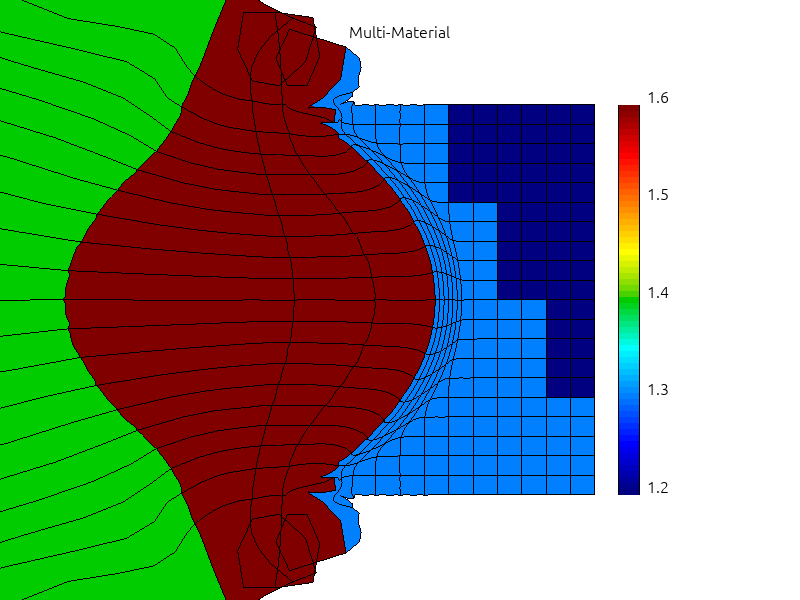
\includegraphics[width=0.3\textwidth]{../../figs_NTH/results/OmegaLaser/material_77.png}
	%&
	%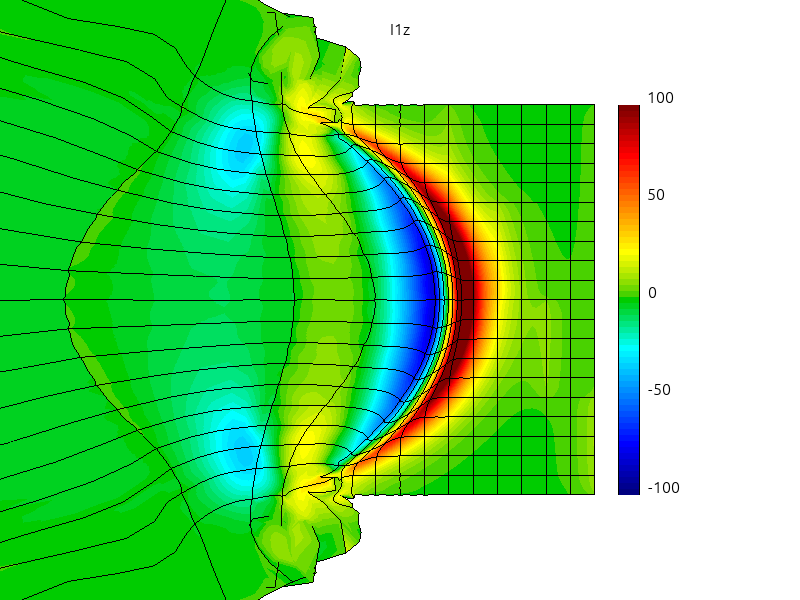
\includegraphics[width=0.3\textwidth]{../../figs_NTH/results/OmegaLaser/nonlocalI1z_77.png}
	%&
	%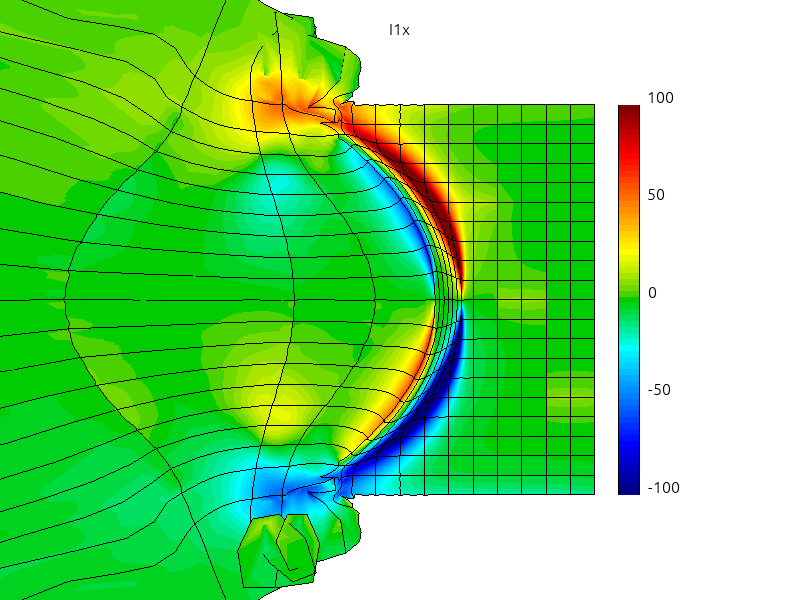
\includegraphics[width=0.3\textwidth]{../../figs_NTH/results/OmegaLaser/nonlocalI1x_77.png}
	%\end{tabular}
	%\end{center}
	%\end{figure}
	\begin{tabular}{c}	
	LLNL - ClubMED,\\
	Livermore, CA,\\
	Jan 7, 2019 
	\end{tabular}
}
%\date{COST Working Group Meeting\\
%Advanced X-ray spatial and temporal metrology\\
%July 9-10, 2015, Madrid}      

\defbeamertemplate*{footline}{miniframes theme}%{shadow theme}
{%
  \leavevmode%
  \hbox{\begin{beamercolorbox}[wd=.5\paperwidth,ht=2.5ex,dp=1.125ex,leftskip=.3cm plus1fil,rightskip=.3cm]{author in head/foot}%
    \usebeamerfont{author in head/foot}\insertframenumber\,/\,\inserttotalframenumber\hfill\insertshortauthor
  \end{beamercolorbox}%
  \begin{beamercolorbox}[wd=.5\paperwidth,ht=2.5ex,dp=1.125ex,leftskip=.3cm,rightskip=.3cm plus1fil]{title in head/foot}% 
    \usebeamerfont{title in head/foot}\insertshorttitle% 
  \end{beamercolorbox}}%
  \vskip0pt%
}      
      
\begin{document}
\begin{frame}
 \titlepage
\end{frame}

\begin{frame}
  \tableofcontents
\end{frame}

\section{Introduction to Nonlocal Magneto-Hydrodynamic model (Nonlocal-MHD)}

\subsection{Radiation-Hydrodyanmics}

\subsection{Nonlocal electron transport}
\newcommand{\edf}{\colorimportant{f}}
\begin{frame}
\begin{center}
{\large Radiation-Hydrodynamic model of plasma}
\begin{block}{Boltzmann transport equation}
\begin{equation}
  \frac{\partial \edf}{\partial t} + 
  \vect{v}\cdot\nabla_x \edf + \frac{q_e}{m_e}\left(\vect{E}
  +\frac{\vect{v}}{c}\times\vect{B}\right)\cdot
  \nabla_{\vect{v}} \edf 
  = 
  \sigma \nabla_{\vect{v}}\cdot\int 
  \frac{|\vect{v}-\vect{v}'|^2\matr{I} - (\vect{v}-\vect{v}')\otimes 
  \vect{v}-\vect{v}')}{|\vect{v}-\vect{v}'|^3}
  \big(\nabla_{\vect{v}} \edf(\vect{v}) f(\vect{v}') - 
  \edf(\vect{v}) \nabla_{\vect{v}} f(\vect{v}')\big) \dI \vect{v}'
  \nonumber
  %C(\edf, \edf)
  %\nonumber
\end{equation}
\end{block}
\begin{block}{Fluid equations in Lagrangian frame}
\begin{eqnarray}
	\frac{\dI \rho}{\dI t} &=& - \rho \nablax\cdot\vect{U}%\, ,
	\label{lagrange_ei_mass_equation} \nonumber\\
	\rho \frac{\dI \vect{U}}{\dI t} 
	&=& \nablax\cdot\matr{\sigma}%\, ,
	\label{lagrange_ei_momentum_equation} \nonumber\\
	\rho\frac{\dI \varepsilon}{\dI t} &=& 
	\matr{\sigma}:\nablax\vect{U}
	- \nablax\cdot\left(\vect{q}_e + \vect{q}_R \right)%\, ,
	\label{lagrange_i_energy_equation} \nonumber
\end{eqnarray}
\end{block}
\begin{block}{Microscopic closure}
\begin{eqnarray}
	\matr{\sigma} &=& -\rho
	\int (\vect{v}-\vect{U})\otimes
	(\vect{v}-\vect{U})\, \edf\, \dI \vect{v}^3 \approx -\matr{I} p 
	+ \tilde{\matr{\sigma}}(\nabla \vect{U})
	\label{stress_tensor}\nonumber\\
	\vect{q}_e &=& \frac{\rho}{2} 
	\int |\vect{v} - \vect{U}|^2
	(\vect{v}-\vect{U})\, \edf\, \dI \vect{v}^3 \approx 
	\frac{\rho}{2} 
	\int_{4\pi}\vect{n}\int_0^\infty 
	|\vect{v}|^5 \edf\, \dI |\vect{v}|\, \dI \vect{n}
	\approx -\kappa(T^{2.5})\nabla T 
	\label{heat_flux_vector} \nonumber \\
	\vect{q}_R &=& \int_{4\pi} \vect{n} \int_\nu I^{~p}_\nu\, \dI \nu\, 
	\dI \vect{n} \approx - \int_\nu \frac{c}{\chi_\nu} \nabla ( f_\nu E_\nu) 
    \, \dI \nu
	\label{radiation_flux_vector} \nonumber
\end{eqnarray}
\end{block}
\end{center}
\end{frame}

\begin{comment} % SH
\begin{frame}
\begin{center}
Spitzer-Harm electron diffusion
\begin{block}{BGK collision operator}
\begin{eqnarray}
  C_{ei}(f^e, f^i)&\stackrel{m_e/m_i}{\approx}& 
  \sigma \nabla_v\cdot\left(\frac{1}{v}
  \left( \matr{I} - \frac{\vect{v}\otimes\vect{v}}{v^2}\right)\cdot\nabla_v 
  f^e\right)
  \nonumber\\
  &\stackrel{\text{spher}}{\approx}& \frac{\sigma}{v^3}
  \frac{1}{\sin(\phi)}\left[\frac{\partial}{\partial \phi}
  \left(\sin(\phi)\frac{\partial f^e}{\partial \phi}\right) 
  + \frac{1}{\sin(\phi)}\frac{\partial^2f^e}{\partial \theta^2}\right] 
  \nonumber \\
  &\stackrel{f^0 + f^1\cos(\phi)}{\approx}& 
  - \frac{2 \sigma}{v^3} f^e_1\cos(\phi) = 
  2 \nu_{ei} \left(f^e_0  - f^e\right) \nonumber
\end{eqnarray} 
\end{block}
Then, the~electron distribution function can be governed by the~BGK Boltzmann transport equation
\begin{equation}
  %\frac{1}{|\vect{v}|}\frac{\partial f^e}{\partial t} + 
  \vect{n}\cdot\nabla_x f^e + \frac{q_e}{m_e |\vect{v}|}\vect{E}\cdot
  \nabla_{\vect{v}} f^e 
  = 
  \frac{2 (f_{MB}(|\vect{v}|, T_e) - f^e)}{\lambda_{ei}}\, , 
  \nonumber
\end{equation}
where $f_{MB}$ is the~Maxwell-Boltzmann equilibrium distribution and 
$\lambda_{ei}$ the~electron mean free path when scattered on ions.
%\begin{eqnarray}
%  \frac{1}{\bar{v}}\frac{\partial I^e}{\partial t} + \vect{n}\cdot\nabla I^e 
%  &=& 
%  \frac{\sigma^e T_e - I^e}{\lambda^e}\, , 
%  \nonumber
%  \\
%  \vect{q}_e &=& \int_{4\pi}\vect{n}\, I^e\, \dI\vect{n}\,  ,
%  \nonumber
%\end{eqnarray}
\begin{block}{Chapman-Enskog approximation in small parameter $\lambda_{ei}$}
\begin{equation}
 f^e = f_0 + \lambda_{ei} f_1 + O({\lambda_{ei}}^2) \approx 
 f_{MB}(|\vect{v}|, T_e)
 - f_{MB}(|\vect{v}|, T_e) g(\bar{Z})
   \left(\frac{|\vect{v}|^2}{2 v_{T_e}^2} - 4\right)
    \vect{n}\cdot\frac{\lambda_{ei}\nabla T_e}{T_e}\nonumber
\end{equation}
\begin{equation}
  \rightarrow \vect{q}_{SH} = \kappa_{SH}\, T_e^{\frac{5}{2}}\, \nabla T_e
  \nonumber 
\end{equation}
%$I \approx \sigma T_e - \lambda \vect{n}\cdot
%  \nabla \left(\sigma T_e\right) + O(\lambda^2)$ 
%$\rightarrow \vect{q} \approx - \lambda \sigma \nabla T_e$ 
\end{block}
\begin{equation}
	\frac{\lambda_{ei} f_1}{f_0} = 0.25
	\left(\frac{|\vect{v}|^2}{2 v_{T_e}^2} - 4\right)
	\vect{n}\cdot\frac{\lambda_{ei}(|\vect{v}|^4)\nabla T_e}{T_e} < 0.1
	\quad\longrightarrow\quad \text{Kn}^e = \frac{\lambda_{ei}\nabla T_e}{T_e} 
	< 7.5\times10^{-4}
	\nonumber \label{SH_limit}
\end{equation}
\end{center}
\end{frame}
\end{comment} % SH

\newcommand{\fsize}{0.335}
\newcommand{\ffsize}{0.33}

\renewcommand{\vect}[1]{\boldsymbol{#1}}
\renewcommand{\matr}[1]{\mathbf{#1}}
\renewcommand{\dI}{\text{d}}
\newcommand{\pdv}[2]{\frac{\partial{#1}}{\partial{#2}}}
\newcommand{\odv}[2]{\frac{\dI #1}{\dI #2}}
\newcommand{\ddv}[2]{\odv{#1}{#2}}
%\renewcommand{\ddv}[2]{\frac{\Delta #1}{\Delta #2}}
\newcommand{\nue}{\nu_{e}}
\newcommand{\nutot}{\nu_{t}}
\newcommand{\vmag}{v}
\newcommand{\vn}{\vect{n}}
\newcommand{\E}{\vect{E}}
\newcommand{\B}{\vect{B}}
\newcommand{\tE}{\vect{\tilde{E}}}
\newcommand{\tB}{\vect{\tilde{B}}}
\newcommand{\qe}{q_e}
\newcommand{\me}{m_e}
\newcommand{\fM}{f_M}
\newcommand{\fzero}{f_0}
\newcommand{\vfzero}{\vect{f}_0}
\newcommand{\fone}{\vect{f}_1}
\newcommand{\SM}{\vect{S}_M}
\newcommand{\MI}{\matr{I}}
\newcommand{\MA}{\matr{A}}
\newcommand{\intO}{\int_{\Omega}}
\newcommand{\IM}{\boldsymbol{\mathcal{M}}}
\newcommand{\ID}{\boldsymbol{\mathcal{D}}}
\newcommand{\IV}{\boldsymbol{\mathcal{V}}}
\newcommand{\IB}{\boldsymbol{\mathcal{B}}}
\newcommand{\acl}{\vect{M}_{\left(\fone/\fzero\right)}}


%\subsection{Nonlocal transport in MHD}
\newcommand{\ftwo}{\boldsymbol{f}_2}
\newcommand{\pv}{\frac{\partial}{\partial v}}
\newcommand{\nuee}{\nu_{ee}}
\newcommand{\nut}{\nu_{tot}}

\begin{frame}
\begin{center}
{\large Nonlocal electron transport $\&$ Maxwell equations}  
\begin{block}{AWBS electron transport equation}
\begin{equation}
  %\frac{1}{|\vect{v}|}\frac{\partial f}{\partial t} + 
  \vect{v}\cdot\nabla_{\vect{x}} f +
  \left( \vect{E} + \vect{v}\times\vect{B}\right)\cdot\nabla_{\vect{v}} f
  = 
  v \frac{\nu_e}{2} \frac{\partial }{\partial v}\left(f - f_{MB}(T_e)\right)
  + \left(\nu_{ei} + \frac{\nu_e}{2}\right) \left(f_0 - f\right)
  \nonumber
\end{equation}
\end{block}
\begin{equation}
  \frac{\partial f}{\partial t} + 
  \vect{v}\cdot\nabla_{\vect{x}} f +
  \left( \vect{E} + \vect{v}\times\vect{B}\right)\cdot\nabla_{\vect{v}} f
  = 
  v \frac{\nu_e}{2} \frac{\partial }{\partial v}
  \left( F(f_0) f_0 + D(f_0)\frac{\partial f_0}{\partial v}\right)
  + \nu_{ei} \left(f_0 - f\right)
  \nonumber
\end{equation}
\begin{block}{Generalized Ohm's law vs. nonlocal Ohm's law}
\begin{eqnarray}
  %\vect{E} + \frac{v_i}{c}\times\vect{B} &=&  
  \vect{E} &=&  
  \left(\vect{R}_T -\nabla p_e\right)\quad~~ + ~\quad\qquad 
  \frac{\vect{j}}{\sigma}\qquad\quad ~+
  \qquad \vect{j}\times\vect{B}
  \nonumber \\
  \vect{E} \int v \pdv{f_0}{v} v^2\, \dI v 
  &=& 
  \int v^2 \nabla f_0 v^2\, \dI v~~~ +~~  \int v \nu_{ei}\fone v^2\, \dI v 
  ~+~~ \int v \fone\times\vect{B} v^2\, \dI v
  %\\
  %\vect{E}\cdot \sum_{\Delta v^g} \int_{4\pi}\matr{V}_E\cdot\vect{f} 
  %&=& 
  %- \sum_{\Delta v^g} \int_{4\pi} \matr{D}\cdot |\vect{v}|\vect{f}~ 
  %-~ \sum_{\Delta v^g} \int_{4\pi} 
  % k_{|\vect{v}|}\matr{M}\cdot |\vect{v}| \vect{f}
  %~-~ \sum_{\Delta v^g} \int_{4\pi} 
  % \matr{B}\times\matr{V}_B\cdot |\vect{v}| \vect{f} 
  %\nonumber 
\end{eqnarray}
\end{block}
\begin{eqnarray}
  \nabla\times\vect{E} &=& -\frac{1}{c}\frac{\partial \vect{B}}{\partial t}
  \quad\qquad (\text{life of magnetic field}~\vect{B}~\text{in fluid frame}) 
  \nonumber \\
  \nabla\times\vect{B} &=& \frac{4\pi}{c}
  \vect{j}\qquad\qquad\,\, (\text{quasi-neutrality} 
  \nabla\cdot\vect{j} = 0) 
  \nonumber
  \\
  \vect{j} &=& C(\vect{E}, f) \qquad\quad (\text{from nonlocal electron transport  model (1)})
  \nonumber
\end{eqnarray}
%Applying generalized Ohm's and Ampere's laws, we get
%\begin{equation}
%  %\nabla\times\tilde{\vect{E}} = 
%   \nabla\times\vect{E} = 
%  \nabla\times\left(
%  \frac{1}{e n_e}\left(\vect{R}_T -\nabla p_e\right) + 
%  \frac{c}{e n_e \sigma 4\pi}\nabla\times\vect{B} 
%  - \frac{\tilde{\vect{j}}}{e n_e \sigma} + 
%  \frac{1}{e n_e c}\vect{j}\times\vect{B}\right)
%  \nonumber
%\end{equation}

%\begin{block}{Maxwell Equations for Hydrodynamics - dynamo equation for 
%nonlocal magnetic field source}
%\begin{equation}
%  \frac{1}{c}\frac{\partial \vect{B}}{\partial t} = 
%  - \nabla\times\frac{1}{e n_e c}\vect{j}\times\vect{B}
%  - \nabla\times\frac{c}{e n_e \sigma 4\pi}\nabla\times\vect{B}
%  - \nabla\times \left(
%  \frac{\sum_{\Delta v^g} \int_{4\pi} \matr{D}\cdot |\vect{v}|\vect{f}}
%  {\sum_{\Delta v^g} \int_{4\pi}\matr{V}_E\cdot\vect{f}}\right)
%  \nonumber
%\end{equation}
%\end{block}
%\let\thefootnote\relax\footnote{Kingham and Bell PRL 2002}
\end{center}
\end{frame}

\begin{comment} % NonlocalRadHydro
\begin{frame}
\begin{center}
{\large Thermal Radiative Transfer}
\begin{block}{Radiation transport equation}
The~radiation intensity $I_\nu(\vect{x}, \vect{n})$ representing photons of frequency $\nu$ obeys the~equation
\begin{equation}
  \vect{n}\cdot\nabla I_\nu = \eta_\nu - \chi_\nu I_\nu , 
  \nonumber \label{eq:RT}
\end{equation}
where \textit{emmisivity} $\eta_\nu(\rho, T)$ and absorptivity 
$\chi_\nu(\rho, T)$ are considered to be isotropic.
\end{block}
\begin{eqnarray}
  \nabla \cdot \vect{q}_\nu &=& 4\pi\eta_\nu - \chi_\nu E_\nu  \nonumber \\
  \nabla \cdot \matr{P}_\nu &=& -\frac{\chi_\nu}{c}\vect{q}_\nu \nonumber
\end{eqnarray}
\begin{block}{Radiation diffusion}
In the~case of low anisotropy pressure tensor can be approximated as
$\matr{P}_\nu = \matr{I} f_\nu E_\nu$ and the~radiation field can be modeled by
\begin{equation}
  \nabla \cdot \left( \frac{c}{\chi_\nu} \nabla ( f_\nu E_\nu) \right) = 
  \chi_\nu E_\nu - 4\pi\eta_\nu , 
  \nonumber
\end{equation}
where the~lowest anisotropy approximation 
$\tilde{I}_\nu(\vect{x}, \vect{n}) = I^0_\nu(\vect{x}) 
+ \vect{n}\cdot\vect{I}^1_\nu(\vect{x})$ 
corresponds to the~\textit{variable Eddington factor} 
$f_\nu = \frac{1}{3}$.
\end{block}
\end{center}
\let\thefootnote\relax\footnote{D. Mihalas and B. Mihalas, Foundations of Radiation Hydrodynamics 
(Oxford University Press, New York, 1985).}
\end{frame}

\subsection{Nonlocal Magneto-Hydrodynamic model}
\begin{frame}
\begin{center}
{\large Nonlocal Magneto-Hydrodynamic model}
%\myheading{Radiative Fluid Model of Laser Plasma}
%Conservation of mass $\rho$, momentum $\rho \vect{u}$, 
%and energy $\varepsilon_e+\varepsilon_i+\epsilon_R$ of radiation field 
%and plasma fluid, 
%where the inverse-bremsstrahlung deposition of laser electric
%field $\vect{E}_L$ heats the target, read 
\begin{eqnarray}
 \frac{\dI \rho}{\dI t} &=& - \rho\nabla\cdot\vect{u}\, , 
 \nonumber\\ 
 \rho\, \frac{\dI \vect{u}}{\dI t} &=& - \nabla (p_i + p_e + p_{\vect{B}}) \, , 
 \nonumber\\   
 \rho \left(\frac{\partial \varepsilon_i}{\partial T_i}\frac{\dI T_i}{\dI t} 
 +\frac{\partial \varepsilon_i}{\partial \rho}\frac{\dI \rho}{\dI t}\right)
 &=& 
 - p_i\nabla\cdot\vect{u} - G(T_i - T_e)\, , 
 \nonumber\\
 \rho \left(\frac{\partial \varepsilon_e}{\partial T_e}\frac{\dI T_e}{\dI t}
 +\frac{\partial \varepsilon_e}{\partial \rho}\frac{\dI \rho}{\dI t}\right)
  %+ \frac{\dI \epsilon_R}{\dI t} 
  &=& 
 - p_e \nabla\cdot\vect{u} - \nabla\cdot\left(\vect{q}_e+\vect{q}_R \right) + 
 G(T_i - T_e) + Q_{\text{IB}}(\vect{E}_L)\, , 
 \nonumber
\end{eqnarray}
the quantities $\frac{\partial \varepsilon}{\partial \rho} =
\frac{\partial f}{\partial \rho}
- T \frac{\partial^2 f}{\partial \rho \partial T}$, 
$\frac{\partial \varepsilon}{\partial T} = 
-T \frac{\partial^2 f}{\partial T^2}$, 
$p = \rho^2 \frac{\partial f}{\partial \rho}$, 
$G = \rho\frac{\partial \varepsilon_e}{\partial T_e} \nu_{ei}$ 
provides our HerEOS equation of state.
\footnote{M. Zeman, M. Holec, P. Vachal, "HerEOS: a Framework for Consistent Treatment of the Equation of State in ALE Hydrodynamics",\\ 
\textit{Comp. Math. Appl.}, submitted (2017).}
%and depend on ion and electron free energies $f_i(\rho, T_i)$, 
%$f_e(\rho, T_e)$ locally. 

\begin{tabular}{c|c}
\hline \\

\begin{pcolumn}{0.42}
Nonlocal transport of photon intensity 
$I^p=\int_\nu f^p\, \frac{h^4\nu^3}{c^2}\, \dI\nu$
\begin{equation}
  %\frac{1}{c}\frac{\partial I^p}{\partial t} + 
  \vect{n}\cdot\nabla I^p = 
  \frac{a T_e^4 - I^{\, p}}{\lambda^p}\,  \label{photon_transport_equation} 
  \nonumber
\end{equation}
%Photon transport equation using Bhatnagar-Gross-Krook collision operator and related closure via radiation energy density
%and radiation energy density flux for hydro
Radiation closure relations
\begin{equation}
  %\epsilon_R &=& \frac{1}{c}\int_{4\pi} I^{\, p}\, \dI\vect{n}\, \nonumber \\ 
  \vect{q}_R = \int_{4\pi}\vect{n}\, I^{\, p}\, \dI\vect{n}
  \xrightarrow{diffusive} \nabla\cdot\vect{q}_R  = 
  - \nabla\cdot\left( \frac{c}{3 \chi_R}\, \nabla E\right) 
  \,  \nonumber\label{rad_momentum} 
  %\matr{P} &=& \frac{1}{c}\int_{\nu}\int_{4\pi}\vect{n}\vect{n}\, \cInun\, \dI\vect{n}\, \dI\nu\, , \label{rad_stress} 
\end{equation}
\end{pcolumn}
&
\begin{pcolumn}{0.5}
Nonlocal transport of electrons
\begin{equation}
  %\frac{1}{|\vect{v}|}\frac{\partial f}{\partial t} + 
  \vect{v}\cdot\nabla_{\vect{x}} f +
  \left( \vect{E} + \vect{v}\times\vect{B}\right)\cdot\nabla_{\vect{v}} f
  = 
  v \frac{\nu_e}{2} \frac{\partial }{\partial v}\left(f - f_{MB}(T_e)\right)
  + \left(\nu_{ei} + \frac{\nu_e}{2}\right) \left(f_0 - f\right)
  \nonumber
\end{equation}
%Photon transport equation using Bhatnagar-Gross-Krook collision operator and related closure via radiation energy density
%and radiation energy density flux for hydro
Electron closure relations
\begin{eqnarray}
  %\varepsilon^e &=& \frac{1}{\bar{|\vect{v}|}}\int_{4\pi} I^e\, \dI\vect{n}\, 
  %\nonumber \\ 
  \vect{q}_e &=& \int\int_{4\pi}\vect{n}\, f^e\, \dI\vect{n}v^5\, \dI v\, 
  \xrightarrow{diffusive} \nabla\cdot\vect{q}_e = 
  - \nabla\cdot\left(\kappa_{SH}\, T_e^{\frac{5}{2}}\, \nabla T_e\right) 
  \nonumber
  \\
  \vect{j} &=& C(\vect{E}, f)
  \xrightarrow{diffusive} \vect{j} = \sigma_e \vect{E}
  \nonumber
  %\\
  %\vect{Kn}^e &=& \frac{\lambda^e \nabla T_e}{T_e}
  %\nonumber 
  %\\
  %\vect{E} &=& \frac{k_B T_e}{q_e}\frac{5}{2}\frac{\nabla T_e}{T_e}
  %\nonumber
  %\matr{P} &=& \frac{1}{c}\int_{\nu}\int_{4\pi}\vect{n}\vect{n}\, \cInun\, \dI\vect{n}\, \dI\nu\, , \label{rad_stress} 
\end{eqnarray}
\end{pcolumn}
\\ \\\hline
\end{tabular} 
\begin{equation}
  \nabla\times\vect{E} = -\frac{1}{c}\frac{\partial \vect{B}}{\partial t},
  \quad
  \nabla\times\vect{B} = \frac{4\pi}{c} \vect{j}
  \nonumber
\end{equation}
\end{center}
\end{frame}
\end{comment} % NonlocalRadHydro

\begin{comment} % CurvelinearHydro
%\section{Nonlocal-MHD code PETE}
\subsection{Hydrodynamics on curvilinear meshes}
%\begin{comment} % RT pics
\newcommand{\RThscale}{0.9}
\begin{frame}
\begin{center}
%{\large Lagrangian High-Order Curvilinear Framework}

 %New generation high-order curvilinear hydrodynamic code
\begin{tabular}{cc}
 \begin{pcolumn}{0.5}
 \begin{varblock}[0.85\textwidth]{Lagrangian High-Order Curvilinear Framework}
 %High-order finite element discretization introduced by 
 %Dobrev, Kolev, and Rieben 
 %
 %Semidiscrete formulation of Euler's equations in Lagrangian frame, 
 %i.e. momentum, energy, and mass conservation, respectively.
 \begin{eqnarray}
   \matr{M}_{\vect{v}}\cdot\frac{\dI \vect{v}}{\dI t} &=& 
     - \matr{F}\cdot\matr{I} \nonumber \\
   \matr{M}_{e}\cdot\frac{\dI \vect{e}}{\dI t} &=& \matr{F}^T\cdot\vect{v} 
     \nonumber \\
   \frac{\dI \vect{x}}{\dI t} &=& \vect{v} \nonumber \\
   \nonumber 
 \end{eqnarray} 
 \let\thefootnote\relax\footnote{Dobrev, Kolev, Rieben, SIAM JSC 34, B606 (2012).}
 \end{varblock}
 \begin{eqnarray}
   \nonumber  
   \\\nonumber\\\nonumber\\\nonumber\\\nonumber\\\nonumber\\\nonumber
   \\\nonumber\\\nonumber\\\nonumber\\\nonumber\\\nonumber\\\nonumber
   \\\nonumber\\\nonumber\\\nonumber\\\nonumber\\\nonumber\\\nonumber
   %\\\nonumber\\\nonumber\\\nonumber\\\nonumber\\\nonumber\\\nonumber
 \end{eqnarray} 
 \end{pcolumn} &
 \includegraphics<1>[height=\RThscale\textheight]{../../figs_NTH/RT_figs/merged_GLVis_s01.png}
 \includegraphics<2>[height=\RThscale\textheight]{../../figs_NTH/RT_figs/merged_GLVis_s20.png}
 \includegraphics<3>[height=\RThscale\textheight]{../../figs_NTH/RT_figs/merged_GLVis_s40.png}
 \includegraphics<4>[height=\RThscale\textheight]{../../figs_NTH/RT_figs/merged_GLVis_s59.png}
\end{tabular}
 %\includegraphics<1>[height=\hscale\textheight]{../RT_figs/merged_GLVis_s01.png}
 %\includegraphics<2>[height=\hscale\textheight]{../RT_figs/merged_GLVis_s10.png}
 %\includegraphics<3>[height=\hscale\textheight]{../RT_figs/merged_GLVis_s20.png}
 %\includegraphics<4>[height=\hscale\textheight]{../RT_figs/merged_GLVis_s30.png}
 %\includegraphics<5>[height=\hscale\textheight]{../RT_figs/merged_GLVis_s40.png}
 %\includegraphics<6>[height=\hscale\textheight]{../RT_figs/merged_GLVis_s50.png}
 %\includegraphics<7>[height=\hscale\textheight]{../RT_figs/merged_GLVis_s60.png}
 %\includegraphics<8>[height=\hscale\textheight]{../RT_figs/merged_GLVis_s70.png}
 %\includegraphics<9>[height=\hscale\textheight]{../RT_figs/merged_GLVis_s79.png}
\end{center}
\end{frame}
\end{comment} % CurvelinearHydro

\begin{frame}
\begin{center}
{\Huge \textit{Nonlocal-MHD} $\iff$ aiming HIGH}

\begin{tabular}{c}
\includegraphics<1>[width=0.4\textwidth]{../figures/Ali_aiming_high.png}
\includegraphics<2>[width=0.7\textwidth]{../figures/getting_high.png}
\includegraphics<3>[width=0.4\textwidth]{../figures/being_high.png}
\end{tabular}

Height 250 m, overhang 40 m, Visera, Riglos, Spain.

\end{center}
\end{frame}

\end{document}
